\subsection{Descripci\'on del problema}

Se nos pide resolver el problema de obtener un orden de fabricaci\'on de joyas tal que se minimice la p\'erdida de dinero. Para lograr esto, se sabe que cada joya $j_{i}$ posee un tiempo de fabricaci\'on $t_{i}$ y un valor de devaluaci\'on diario $d_{i}$. \\

Para calcular la p\'erdida dado un orden de fabricaci\'on, se debe calcular la siguiente f\'ormula:

$\sum\limits_{i=0}^n d_{i}*dia\_finalizacion\_joya_{i}$

Donde $n$ es la cantidad de joyas menos uno, y $dia\_finalizacion\_joya_{i}$ es el dia global en el que se termina de fabricar la joya.\\

Por ejemplo, dadas las joyas $j_{0}$, $j_{1}$ y $j_{2}$ con tiempos de fabricaci\'on 3, 5 y 8, y valor de devaluaci\'on 10, 30 y 15 respectivamente, la soluci\'on \'optima ser\'ia el siguiente orden de fabricaci\'on:

\begin{center}
\begin{figure}[h]
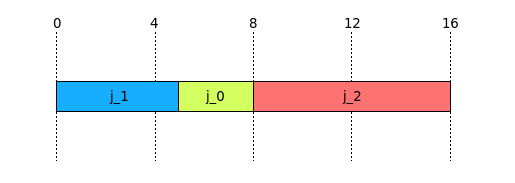
\includegraphics[scale=0.7]{./img/ej2_chart1.png}
\caption{Distribuci\'on de las joyas a fabricar}
\end{figure}
\end{center}

Esta disposici\'on se calcula con la siguiente formula:

$d_{1}*5 + d_{0}*8 + d_{2}*16 = 455$

Se puede comprobar calculando la misma formula para todas las permutaciones posibles del problema que esta es la \'optima: \\

$d_{1}*5 + d_{0}*8 + d_{2}*16 = 455$ \\
$d_{0}*3 + d_{1}*8 + d_{2}*16 = 510$ \\
$d_{2}*8 + d_{0}*11 + d_{1}*16 = 710$ \\
$d_{0}*3 + d_{2}*11 + d_{1}*16 = 675$ \\
$d_{1}*5 + d_{2}*13 + d_{0}*16 = 505$ \\
$d_{2}*8 + d_{1}*13 + d_{0}*16 = 670$ \\

\subsection{Resoluci\'on}

Para resolver el problema se decidio elegir algun tipo de medida de $peso$ para poder clasificar las joyas, donde $peso$ refiere especificamente a la siguiente ecuaci\'on: \\

$peso\_j_{i} = \frac{d_{i} / t_{i}}{\sum\limits_{i=0}^n d_{i} / t_{i}}$

Esta formula entrega un porcentaje de peso relativo de una joya al resto. Una vez medido el peso de todas las joyas, el algoritmo procede a ordenar la fabricaci\'on de las joyas por su peso de mayor a menor. \\

Una descripci\'on del algoritmo en pseudo codigo:

\begin{itemize}
\item Para cada joya, calcular el peso de la joya y guardar el peso en un acumulador
\item Para cada joya, calcular el porcentaje de peso con respecto al resto
\item Ordenar las joyas segun su porcentaje de peso
\end{itemize}

\subsection{Demostraci\'on de la resoluci\'on}

Como se mencion\'o anteriormente, el algoritmo necesita un m\'etodo de clasificaci\'on de las joyas. Como cada joya depende de dos variables (su devaluaci\'on diaria y el tiempo que demora en fabricarse), $d_{i}/t_{i}$ nos entrega la relacion entre estas dos variables. En otras palabras, cuantas unidades de devaluaci\'on se generan por cada unidad de tiempo. \\

Con esa idea, el algoritmo pretende ordenar las joyas de manera tal que la joya con mayor devaluaci\'on por dia sea fabricada primero, entonces se compara que porcentaje sobre el total de las joyas ocupa cada una y se fabrican en orden, de mayor a menor porcentaje de peso.

\subsection{Complejidad del algoritmo}

Analizaremos a continuaci\'on la complejidad del algoritmo propuesto utilizando el pseudo c\'odigo como gu\'ia.

\begin{itemize}
\item poner acumPesos = 0 , $O(1)$
\item para cada  joya en input, $O(n)$
\begin{itemize}
\item poner joya.peso = joya.devaluacion / joya.tiempo\_fabricacion
\item poner acumPesos = acumPesos + peso de la joya
\end{itemize}
	
\item para cada joya en input, $O(n)$
\begin{itemize}
	\item poner joya.porcentaje\_peso = joya.peso / acumPesos, $O(1)$
\end{itemize}

\item ordenar joyas de mayor a menor por joya.porcentaje\_peso , $O(n*log(n))$
\end{itemize}



Notar que n es la cantidad de trabajos/joyas a confeccionar y que se simplific\'o el algoritmo para que fuera m\'as simple ver la complejidad.

Como se puede ver en el seguimiento, la complejidad del algoritmo elegido es O(n*log(n)) ya que es la complejidad predominante.\\

\subsection{Codigo fuente}

\subsection{Casos de prueba}

\subsection{Performance}
